%%%---%%%---%%%---%%%---%%%---%%%---%%%---%%%---%%%---%%%---%%%---%%%---%%%---%%%---%%%---%%%---%%%---%%%---%%%---%%%---%%%---%%%---%%%---%%%---%%%
%
\chapter{Overview of the solution}
%
%%%---%%%---%%%---%%%---%%%---%%%---%%%---%%%---%%%---%%%---%%%---%%%---%%%---%%%---%%%---%%%---%%%---%%%---%%%---%%%---%%%---%%%---%%%---%%%---%%%
This chapter presents the main functionality of the debugging tool in all generalities and presents how it has been integrated with Intellij IDE as a GUI plugin.

%%%---%%%---%%%---%%%---%%%---%%%---%%%---%%%---%%%---%%%---%%%---%%%---%%%---%%%---%%%---%%%---%%%---%%%---%%%---%%%---%%%---%%%---%%%---%%%---%%%
\section{Overview}
%%%---%%%---%%%---%%%---%%%---%%%---%%%---%%%---%%%---%%%---%%%---%%%---%%%---%%%---%%%---%%%---%%%---%%%---%%%---%%%---%%%---%%%---%%%---%%%---%%%
To empower Autumn's parsing library with a proper debugging tool, we developped an IDE plugin designed to be a straple for the developper to interact with the grammar's output and track down errors. During a debugging session, Autumn will attempt to parse the entire input. Weather it is successful or not, it produces a parse tree during its invocation.

\bigskip

The generated parse tree is then passed to the plugin's GUI. Each node of the tree represents the invocation of a single parser and contains information about the circumstances surrounding its invocation that can be used to assess the correctness of its behavior

\bigskip

The tree itself can be seen as a list representing the history of invocation, the first entry being the starting expression. Each entries representing a moment in time during the parse, one can retrace the execution of the entire parse, stepping forward or backward simply by navigating up and down the list. 

\bigskip

The debugging effort can therefore be summurized as a search in a tree of event.


%%%---%%%---%%%---%%%---%%%---%%%---%%%---%%%---%%%---%%%---%%%---%%%---%%%---%%%---%%%---%%%---%%%---%%%---%%%---%%%---%%%---%%%---%%%---%%%---%%%
\subsection{Why not a ``normal'' debuger ?}
%%%---%%%---%%%---%%%---%%%---%%%---%%%---%%%---%%%---%%%---%%%---%%%---%%%---%%%---%%%---%%%---%%%---%%%---%%%---%%%---%%%---%%%---%%%---%%%---%%%

From the start, we wanted to create a plugin that would serve as a GUI for our debugger. The original idea was to create a more conventional debuger by overlaying our logic on top of Intellij's general purpose debugger to do achieve a more traditional approach allowing us to step live into the execution. The problem is that Intellij doesn't expose the implementation of its debugger through the plugin interface, making it a much more difficult endeavor. To access the IDE's debugger, one could work directly with the community version of the IDE which is open source, but we decided to stick with our plugin interface.

\bigskip

Facing this problem made us think the solution over in term of practical use. We tried to put ourselves in the shoes of grammar developpers and asked ourselves questions like: 

\begin{itemize}
	\item What problem will I face while developping a grammar ?
	\item What information do I need to track errors down and take decisions ?
	\item How can I get those informations in the simplest possible way ?
\end{itemize}

\subsection{Difficulties of grammar development} 

The most common problem encountered by grammar developpers is to determine why a generated parser incorrectly interprets an input sentence. Generally, an incorrect parse can be reduced to three different cases:

\begin{itemize}
	\item The grammar contains a certain number of wrong production rules that leads to a wrong interpretation of the input.
	\item The input itself contains incorrect parts with respect to the specification of the grammar which in turns lead to a wrong interpretation of the input.
	\item There is a mistake in the definition of some user custom parser.
\end{itemize}

\paragraph{TODO} Having some examples of bad error reporting and highliting the difficulties of grammar debugging here might be a good place

\bigskip

To deal with those issues, the most important properties that we need are :

\begin{itemize}
	\item to able to expose chronologically call sequence of each parser.% This is traditionally done by stepping into the next instruction in traditional debugging. 
	\item the ability to manipulate the input stream and identify what portion of the input a particular parser has matched. Additionally to be able to analyze the parsing behavior at a certain position in the input is also very valuable. %Traditional parsers have no knowledge of input stream manipulation, therefore the only way to accomplish this is to manually step into the code instruction by instruction which is time consumming and inconvenient.
	\item lastly, to be able to inspect the condition of the general parse state during the call of a particular parser. %Similarly to the previous point, traditional parsers have no knowldege about parse state.
\end{itemize}

As we discussed before, general purposed debugger fall short of dealing with those particular points. Indeed, general purpose debuggers don't have any knowledge of input stream manipulation or parse state, therefore the only way to gather those information using a general purposed debugger is to manually step into the code and monitor mentally the mutation of some low level data structures which is far from convenient.

\bigskip

We wanted to be able to observe the flow of execution of the parse at a higher level of abstraction than instruction by instruction. We wanted to be able to travel through time at the parser level, being able to see which parser was called in which order, being able to see where a parse failed and to be able to go back in time to analyze if the condition for it to succeed was theorically met or if the problem came from elsewhere. We wanted to be able to jump immediately to a certain point in the input stream and see how the parser matched a particular portion of it. And finally, we wanted to be able to analyze the parse state at any point during the execution of any parser.

\bigskip

The question was then, instead of enhancing the general debuger with the required abstractions, could we do that in another way ? Our alternate approach proved to be much simpler indeed. By building a parse tree that can be navigated, we meet the first requirement of analyzing the flow or sequence of invocation of the parsers as well as exposing the hierachy of the parsers.

Autumn's formalism can be specified as a ``functional flow'' where one can plug an arbitrary function that consults the input and push the parse forward or fail. The only information required to simulate input stream manipulation is the position in the input that the parser consulted. It is not unreasonable to reccord a single integer for each node of the tree, that leaves the lasst problem of being able to analyze the parse state at any point.

\bigskip

When manipulating the parse state, autumn keep a log of every mutation a parser applied to it. This structure is maintained primarely to revert the mutation a backtracking parser applied to the state. This structure serves our purpose as well, all we have to do is to record the size of the log for each parser. From this information, it is easy to regenerate the parse state as it were during the invocation of a specific parser.

\bigskip

Our alternate solution to traditional debugging is build on this idea, building a parse tree and recording the input position as well as the log size for each parser. Navigating this tree allow us to observe the flow of execution just as we were travelling back and forth through time at the parser's invocation. 
	
	% the syntax tree generated by the parse can by analyze and we can simulate time traveling in the parse execution
%%%---%%%---%%%---%%%---%%%---%%%---%%%---%%%---%%%---%%%---%%%---%%%---%%%---%%%---%%%---%%%---%%%---%%%---%%%---%%%---%%%---%%%---%%%---%%%---%%%
\section{Functionality}
%%%---%%%---%%%---%%%---%%%---%%%---%%%---%%%---%%%---%%%---%%%---%%%---%%%---%%%---%%%---%%%---%%%---%%%---%%%---%%%---%%%---%%%---%%%---%%%---%%%


	\paragraph{Syntax tree}
	Originally, autumn doesn't build a syntax tree like it is generally done in other parsing libraries. Instead it directly generate a abstract syntaxt tree (AST) which contract nodes together to make them easier to read from a human stand-point. Such an AST doesn't represent the grammar as closely as a regular syntax tree as we no longer have a one to one relationship between the grammar rules and nodes of the tree.

	\bigskip

	Having a one to one relationship between the rules of the grammar and the node of the tree is a crutial property for our debugging purpose. Indeed, we navigate through the tree to observe the invocation of the parsers through time, so if a particular node is actually the abstraction of several children parser, it can be that one node doesn't correspond to one rule of the grammar but to several. To be able to tell which one contains errors would be made much more difficult and less relevant.

	\bigskip

	The debugger assumes the task of building the required syntax tree. Since both trees contain essentially the same information, we could easily have had the Autumn's logic build the syntax tree at the same time it does the AST to improve the performances and avoid uneccessary work. Nonetheless, we choose to seperate the debugging logic from autumn's implementation as best we could to minimize coupling between the debugger and Autumn. Autumn's logic doesn't need to build the syntax tree and so this effort should be undertaken only in the debugging context.

	\begin{comment}
		\item Autumn implementation of parser as function -> changed into objects to create hooks for debugger.
		\item neet to rewrite java grammar to reflect changes in the parsers implementation

		\item each node of the syntax tree contains informations about the parse state at the moment of the parser invocation
		\item those information can then be processed and displayed on a GUI for the developper to reason about
		\item ULM chart of the debugger and how it connects to autumn
	\end{comment}



	% We developped a debugger, to do so we had to adapt autumn parsers. Parsers were initially boolean functions, we transformed them into objects that can be manipulated and stored to remember which parsers were called and in which order during runtime
	\paragraph{Gathering relevant information}
	The syntax tree is build implicitely during the invocation of each parser. Every time a parser is called, a new node is create in the tree and some information about the context is recorded within the node. The information reccorded in the node are:
	\begin{itemize}
		\item the \textbf{name of the production rule} the parser is defining, if any. Each production rule being defined by a combination of parsers, some parser are just a part of the definition of such rule.
		\item the \textbf{type of the parser}. (i.e. Seq, Str, \dots)
		\item its \textit{parent} and \textit{children}
		\item and the \textbf{log size} to regenerate the parse state
	\end{itemize}

%%%---%%%---%%%---%%%---%%%---%%%---%%%---%%%---%%%---%%%---%%%---%%%---%%%---%%%---%%%---%%%---%%%---%%%---%%%---%%%---%%%---%%%---%%%---%%%---%%%
\section{Intellij plugin}
%%%---%%%---%%%---%%%---%%%---%%%---%%%---%%%---%%%---%%%---%%%---%%%---%%%---%%%---%%%---%%%---%%%---%%%---%%%---%%%---%%%---%%%---%%%---%%%---%%%

	% All these information can then be displayed on a GUI.

	The plugin we developped is essentially composed of a panel that can be docked on any side of the IDE window, although it is recommanded to dock in at the bottom or on floating on another screen for maximum clarity. Figure \ref{fig:intj_plug} shows how the plugin integrate within the IDE.

	\begin{figure}[h]
		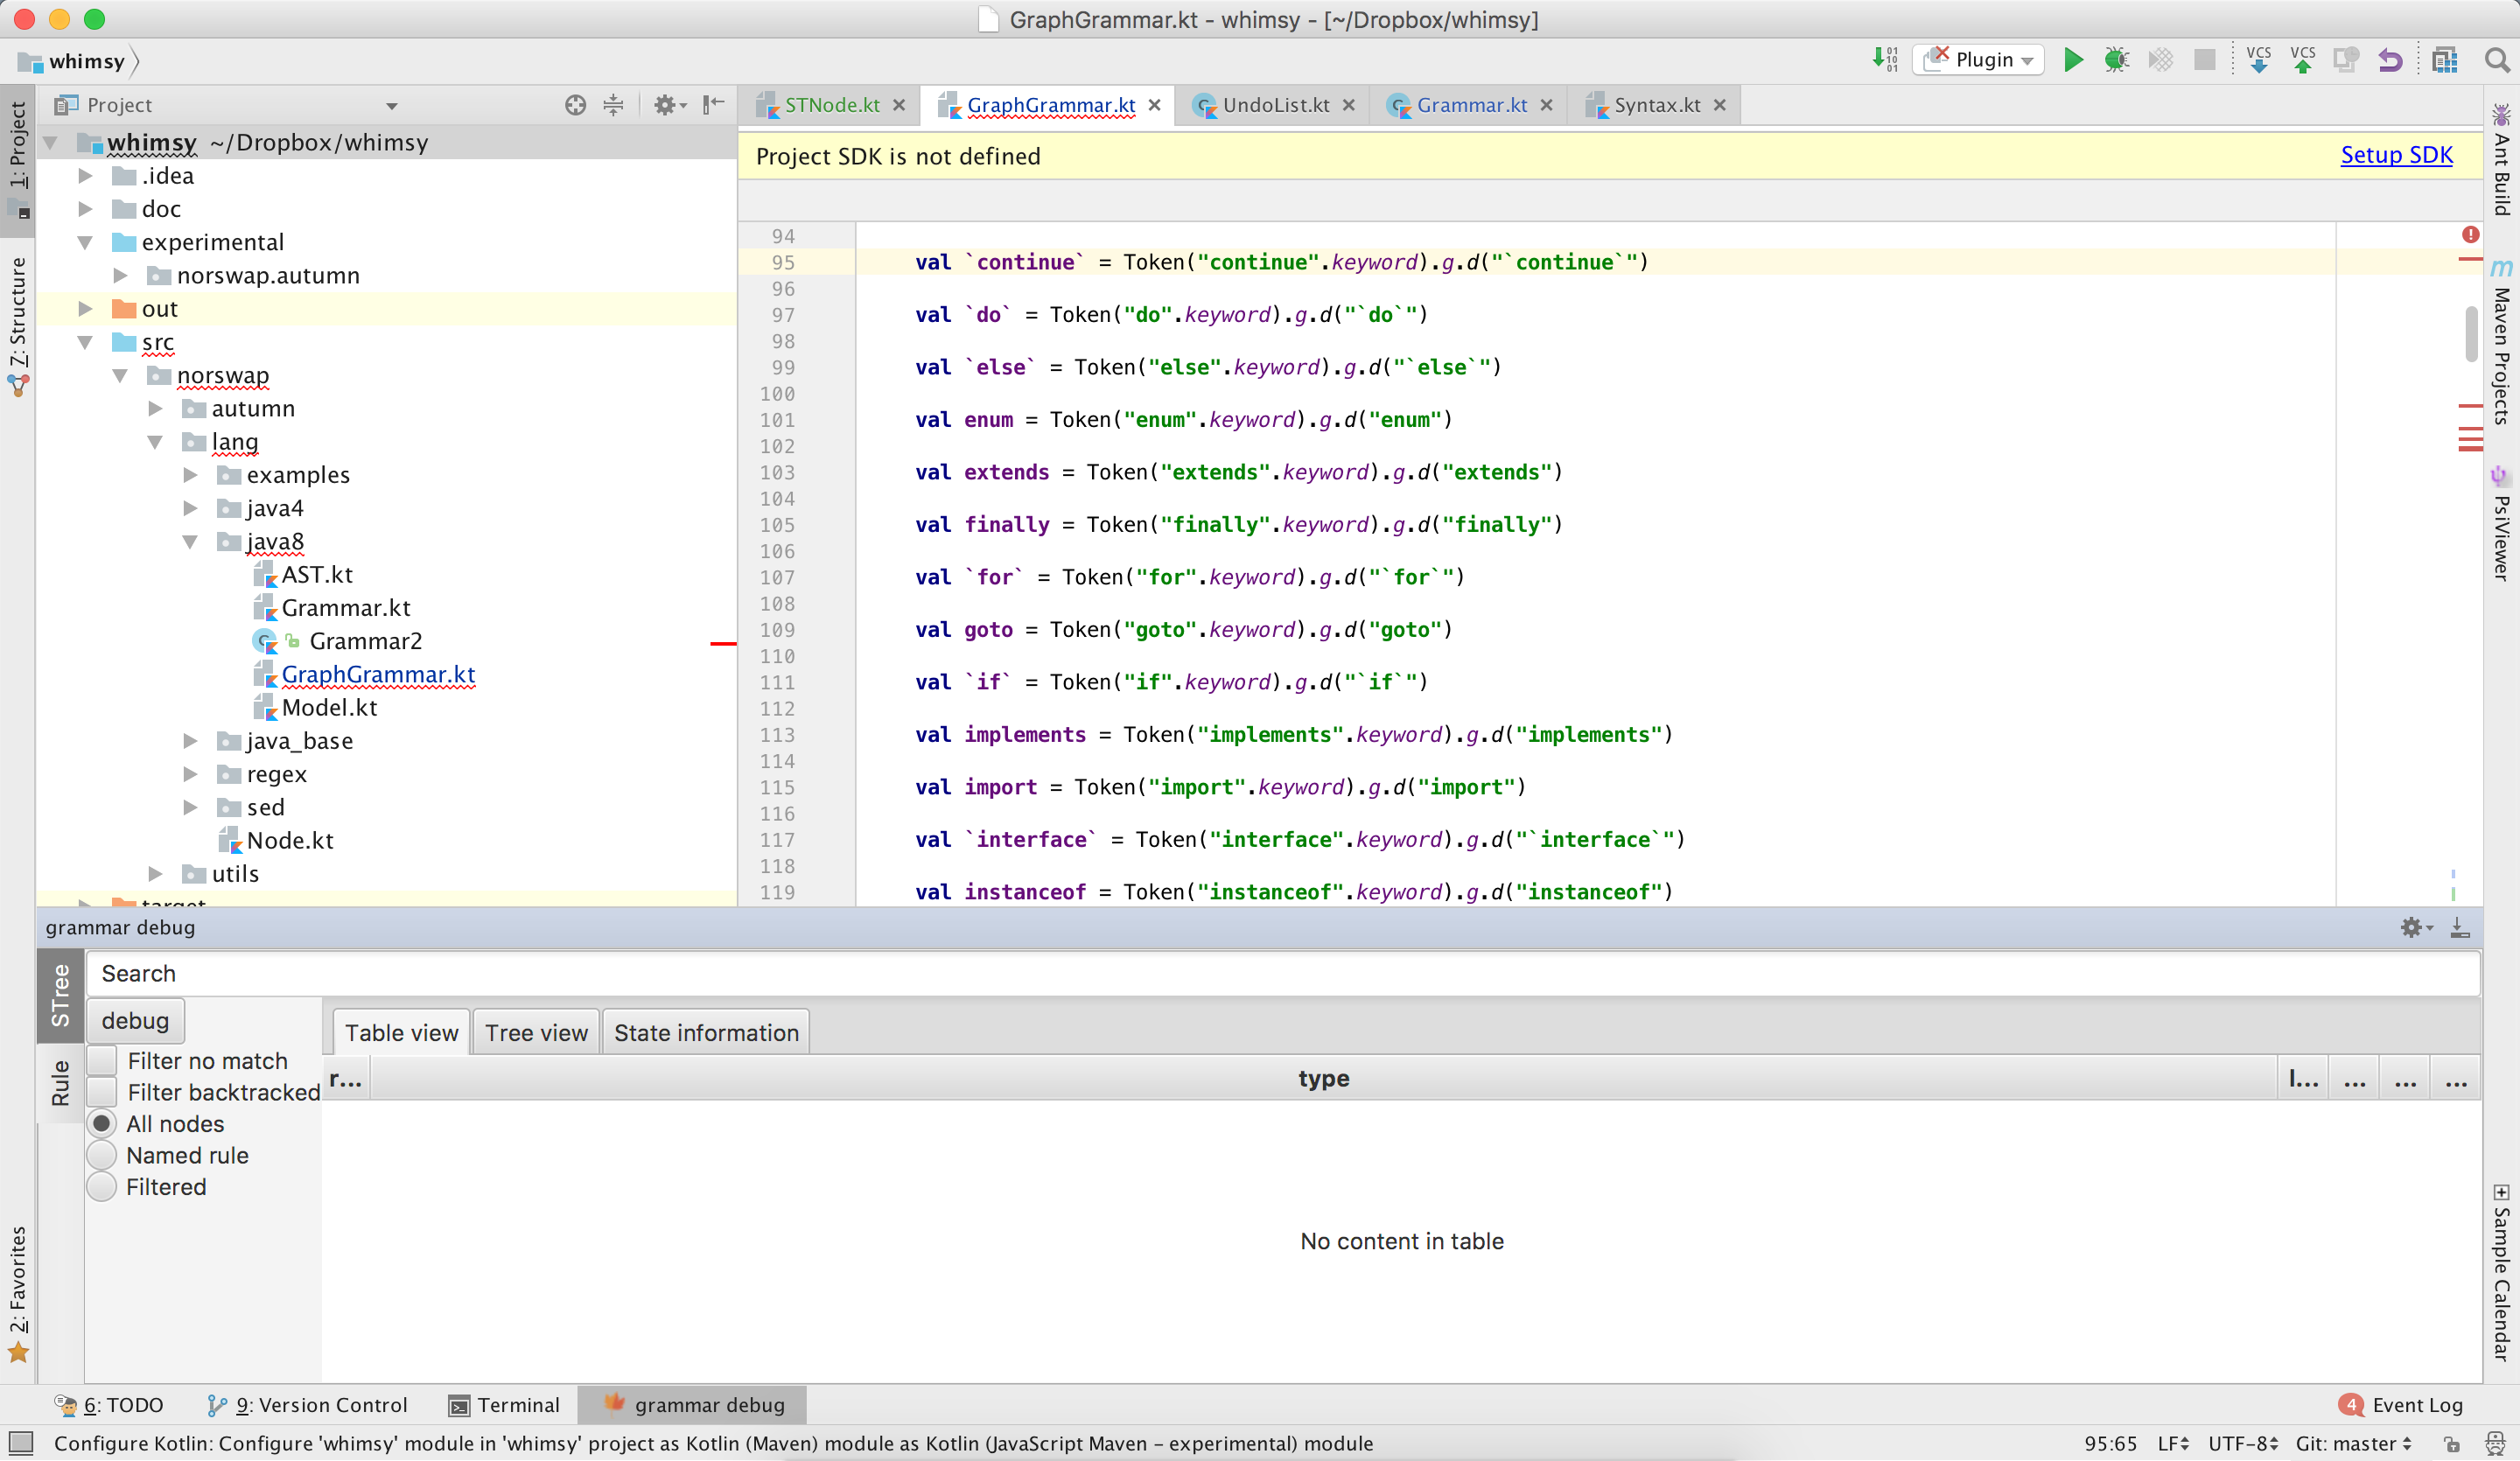
\includegraphics[width=1\textwidth] {ressources/intj_plug}
		\caption{IDE GUI for Autumn's debuggin tool} 
		\label{fig:intj_plug}
	\end{figure}

	The parse tree that has been build can be displayed in two different forms. A table form and a tree form, the former represents the execution trace, it displays each parser in the sequence they were called in a simple list. The later displays the same information as a tree, highlighting the hierachy between parsers.

	\bigskip

	It can be argued that the tree view would be enough and that having a table view would be redundant. While this is true, given the highly recursive nature of grammar rules, navigating the tree can quickly lead to very high level of nesting, while it makes the hierachy between parsers obvious it also makes it more difficult to have a clear image of the sequence of calls. On the other hand, the table view being a simple list makes it really easy to follow the sequence of call one by one, the downside being that it hides the parser hierachy. So even if it can argued that both views are redundant and unecessary, we think that in some cases, it can provide a small improvement in the quality of life of the developper which is what this tool is all about.

	\bigskip

	It can also be argued that this information as is wouldn't be very useful to the developper as it is quiet a dump of information. When trying to debug a grammar, most of the time we are interested in the behavior of a restricted number of rules that we suspect are carrier of mistakes. In traditional debugging, this is done by setting a serie of breakpoints and executing the code. Once the breakpoint occurs, the programmer will generally single step through the code instructions by instructions. In this domain, it is rarely useful to single step through each instructions as you are more interested in the behavior of the rules as a whole rather than the sum of each of its parts.

	\bigskip

	By implementing a serie of filters and search field, one can really easily find the execution of the parser or rule he is interested, from there he can easily navigate the tree up and down to see how the grammar parsed the input around those particular parsers. 

	\paragraph{}

	Note that the plugin can also run as a stand alone application as shown on figure \ref{fig:stand_alone}, albeit some of the functionnalities (those that are tightly coupled to the IDE, like jumping to the rule definition) are disabled. The usefulness of such feature can be critized, but the feature is there and could serve as a starting point to develop a full fledged debugging environment for autumn grammars that are independent from the IDE. 

	\begin{figure}[H]
		\centering
		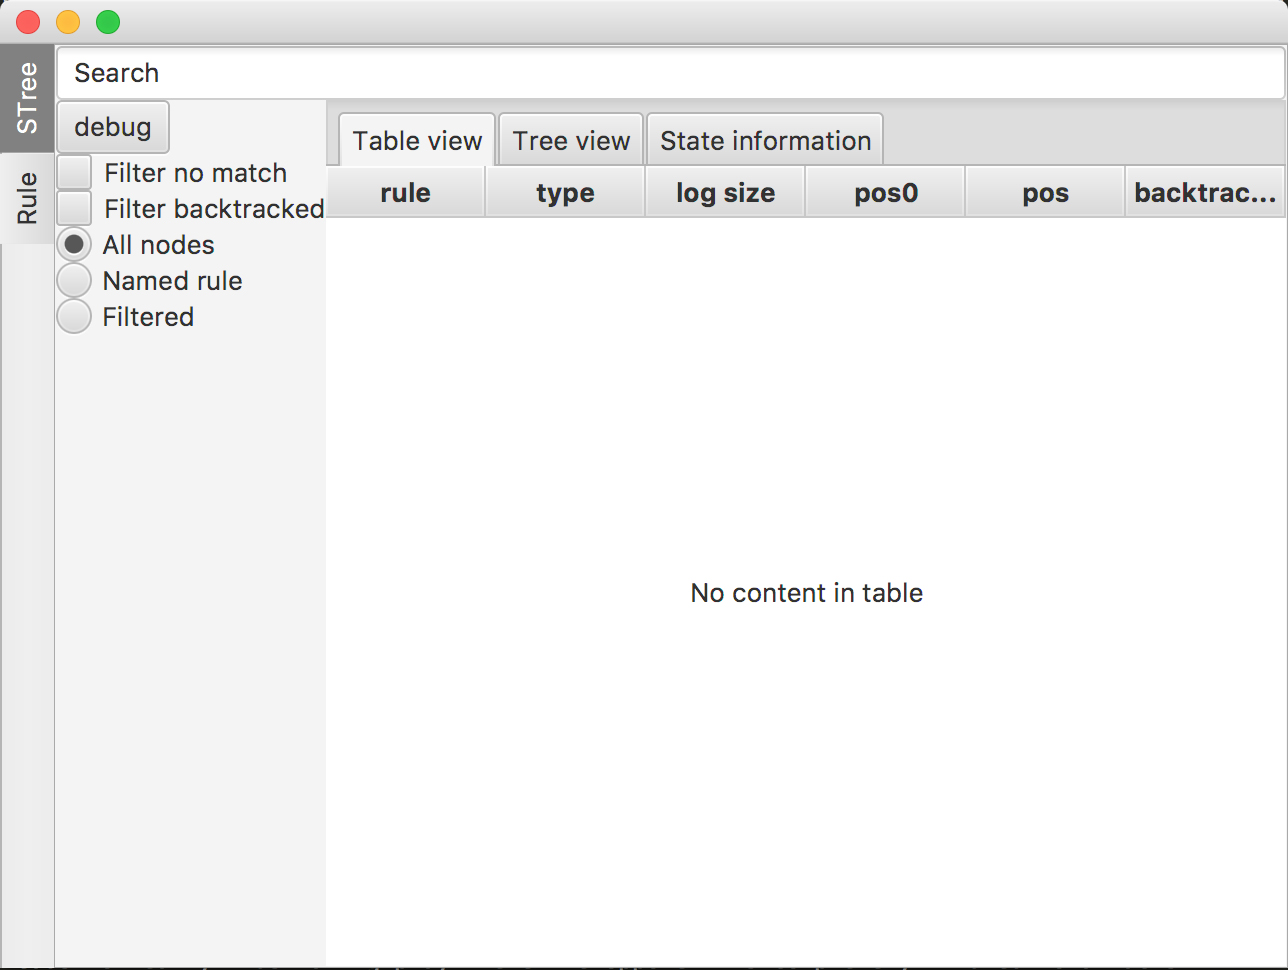
\includegraphics[width=.75\textwidth] {ressources/stand_alone}
		\caption{Stand alone view - the debugger GUI can be executed independetly from the IDE albeit some restrictions} 
		\label{fig:stand_alone}
	\end{figure}





%%%---%%%---%%%---%%%---%%%---%%%---%%%---%%%---%%%---%%%---%%%---%%%---%%%---%%%---%%%---%%%---%%%---%%%---%%%---%%%---%%%---%%%---%%%---%%%---%%%
	\subsection{Views}
%%%---%%%---%%%---%%%---%%%---%%%---%%%---%%%---%%%---%%%---%%%---%%%---%%%---%%%---%%%---%%%---%%%---%%%---%%%---%%%---%%%---%%%---%%%---%%%---%%%
	Let's describe the content of the different views in a little more details.

		\begin{figure}[h]
			\includegraphics[width=1\textwidth] {ressources/stand_alone_detailed}
			\caption{Close up view of the plugin in detail} 
			\label{fig:stand_alone_detailed}
		\end{figure}

		\paragraph{Figure \ref{fig:stand_alone_detailed} presents the different elements of the GUI.}
		\begin{itemize}
			\item 1. Debug button, used to start the debugging process
			\item 2. Filters buttons, used to apply filters to the displayed data
			\item 3. Search field, used to filter the parsers by name
			\item 4. Main information display, 3 tabs are available : Table view, Tree view and finally state view
			\item 5. Side tab panel, used to switch from the main view to the rule view.
		\end{itemize}

		\paragraph{Table view - Execution trace} The table view highlight the execution sequence of the parsers. It is a list countaining the parser calls in chronological order. This view can be considered redundant with the tree view which offer the same information but displayed in a tree fashion. Dispite it's redundancy, it shouldn't be dismissed too eagerly, in a tree view, the potentially high nesting of each nodes can create situation where two chronological consecutive parser calls happen in two very different nesting level making the structure harder to read when one focus on the chronological property of events. This is the reason why we considered this view to be important as well, an example of this view displaying information of a trivial parse can be seen on figure \ref{fig:tableview}

		\paragraph{}

		\begin{figure}[h]
			\centering
			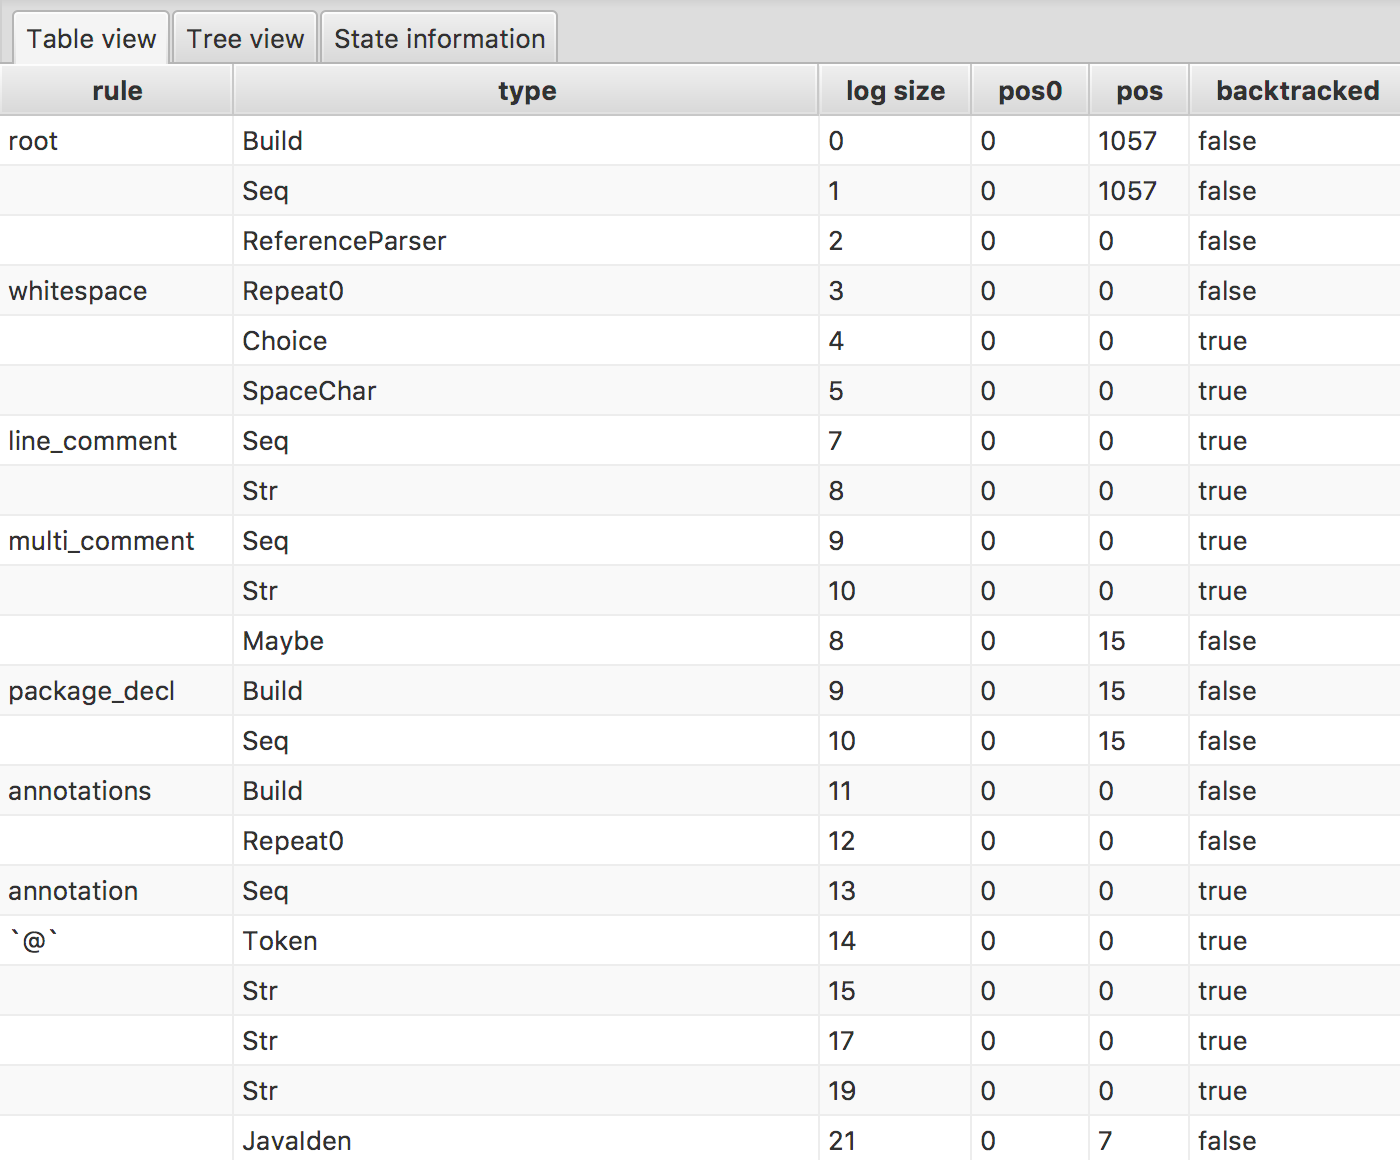
\includegraphics[width=.7\textwidth] {ressources/tableview}
			\caption{Table view: Chronological parser call on a trivial parse example} 
			\label{fig:tableview}
		\end{figure}

		\paragraph{Context menu - Show rule info}


		\paragraph{Tree view - Syntax tree} The tree view displays the data in a tree like structure. It highlights the hierarchy between parsers making it obviously easy to trace where the call comes from. An example of this view can be seen on figure \ref{fig:treeview} for a trivial parse example.
		
		\paragraph{}

		\begin{figure}[h]
			\centering
			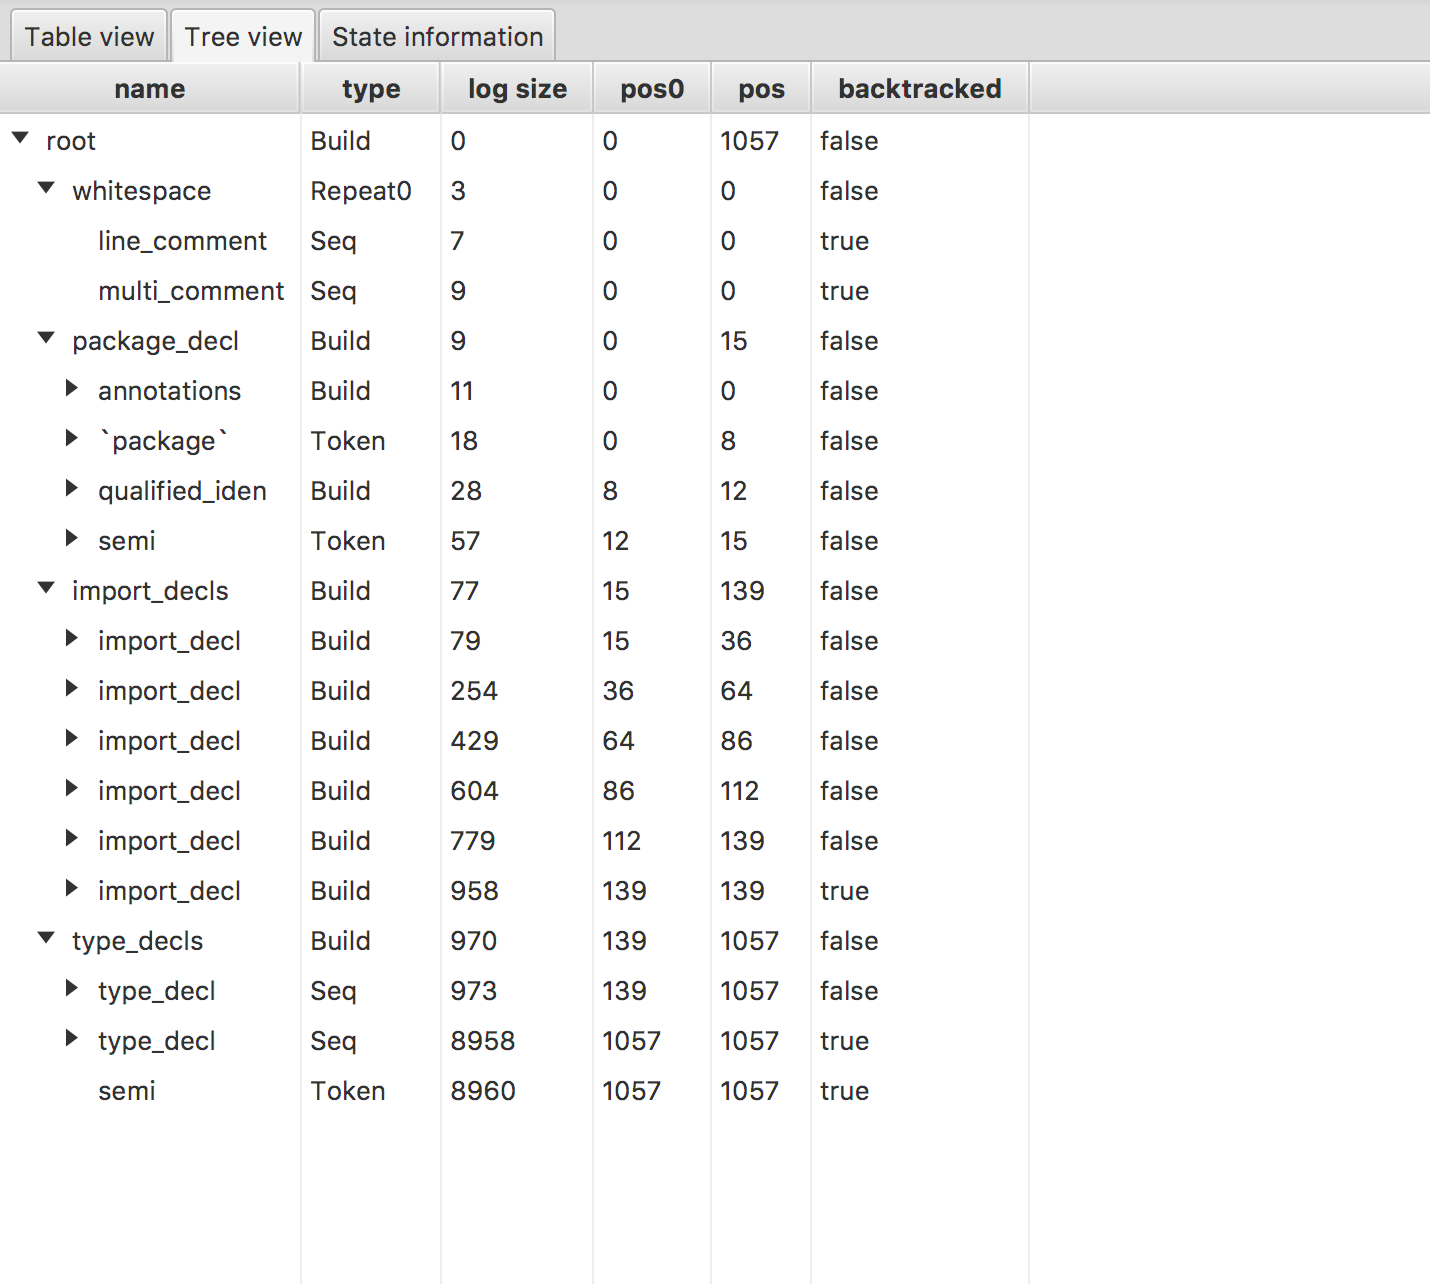
\includegraphics[width=.7\textwidth] {ressources/treeview}
			\caption{} 
			\label{fig:treeview}
		\end{figure}

		\paragraph{Context menu - Set as root}
		\paragraph{Context menu - Set parent as root}
		\paragraph{Context menu - Reset root}
		\paragraph{Context menu - Analyze entry}

		\paragraph{State information} The last tab of the main view's purpose is to display the parse state associated to the parser currently inspected. In the current implementation of Autumn, the parse state is simply used to record the position of the input and the abstract syntax tree built during the parse. Both information are already displayed in the other views, therefore, it doesn't display information for now. This tab remains relevant notherless because users can implement their own structures to store custom parse state providing they respect Autumn's prescription for such structure. Those custom structure could contain relevant information that has not been captured by the other views. The existance of this tab, and a hook that has been implemented in those structure can greatly facilitate the display of such custom information.


		\paragraph{Rule side tab} Finally the side tab displays information about a specific parser we want to anlyze. By double clicking or using the appropriate context menu option in the table or tree view, one can display the definition of the grammar rule as well as the portion of the input that has been matched by the parser. Figure \ref{fig:ruledis} shows an example of that.

		\begin{figure}[h]
			\includegraphics[width=1\textwidth] {ressources/ruledis}
			\caption{Example of grammar rule information and matched input for a particular parser} 
			\label{fig:ruledis}
		\end{figure}

		%%%---%%%---%%%---%%%---%%%---%%%---%%%---%%%---%%%---%%%---%%%---%%%---%%%---%%%---%%%---%%%---%%%---%%%---%%%---%%%---%%%---%%%---%%%---%%%---%%%
		\subsection{Filtering the informations}
		%%%---%%%---%%%---%%%---%%%---%%%---%%%---%%%---%%%---%%%---%%%---%%%---%%%---%%%---%%%---%%%---%%%---%%%---%%%---%%%---%%%---%%%---%%%---%%%---%%%

		\begin{itemize}
			\item all this information is overwhelming and not very useful (like a dump of info)
			\item filter allow to select the relevant informations the user might be reasoning with
			\item filter possibilities
			\item unamed: unamed parser which doesn't match the rule one to one 
			\item backtracked
			\item no match : nodes that didn't match anything in the input but succeded
		\end{itemize}

		%%%---%%%---%%%---%%%---%%%---%%%---%%%---%%%---%%%---%%%---%%%---%%%---%%%---%%%---%%%---%%%---%%%---%%%---%%%---%%%---%%%---%%%---%%%---%%%---%%%
		\subsection{Jump to code}
		%%%---%%%---%%%---%%%---%%%---%%%---%%%---%%%---%%%---%%%---%%%---%%%---%%%---%%%---%%%---%%%---%%%---%%%---%%%---%%%---%%%---%%%---%%%---%%%---%%%

		% Because we don't stop the execution with breakpoints, the user will get the entire execution trace and all the related information with it at once. This can be a little bit overwhelming and therefore defeat the purpose of the debugger. To facilitate the navigation of thoses information we create filtering tools. The user can decide what to display at anytime. The different filters fill in different roles. It is possible to filter the unamed parser which doesn't match the rule one to one to get a ``higher'' level view of the parsing. One can filter out the node that backtracked to see exactly how the input has been matched. Because of the nature of certain parsers, there will be nodes that didn't match anything in the input but succeded anyway and therefore didn't backtracked, those nodes are filterable as well. And finally, because the user might be interested only in the matching of a particular rule or parser, there is a search field in which we can input the name of the parser of interest to filter everything else out.


		%PetitParser is a framework for creating parsers, written in Pharo, that makes it easy to dynamically reuse, compose, transform and extend grammars [28]. A parser is created by specifying a set of grammar productions in one or more dedicated classes. When a parser is instantiated the grammar productions are used to create a tree of primitive parsers (e.g., choice, sequence, negation, etc.); this tree is then used to parse the input. Whereas most parser generators instantiate a parser by generating code, PetitParser generates a dynamic graph of objects. Nevertheless, the same issues arise as with conventional parser generators: generic debuggers do not provide debugging operations at the level of the input (e.g., set a breakpoint when a certain part of the input is parsed) and of the grammar (e.g., set a breakpoint when a grammar production is exercised). Generic debuggers also do not display the source code of grammar productions nor do they provide easy access to the input being parsed.

